\documentclass[10pt]{article}
\usepackage[a4paper,margin=2.2cm]{geometry}
\usepackage{amsmath,amssymb,amsthm,bm}
\usepackage{graphicx,booktabs,xcolor}
\usepackage[font=small,labelfont=bf]{caption}
\usepackage[colorlinks=true,linkcolor=blue!50!black,citecolor=blue!50!black,urlcolor=blue!50!black]{hyperref}

\newtheorem{proposition}{Proposition}
\newtheorem{theorem}{Theorem}
\newtheorem{lemma}{Lemma}
\theoremstyle{remark}
\newtheorem{remark}{Remark}
\theoremstyle{definition}
\newtheorem{assumption}{Assumption}

\newcommand{\Gb}{\bar G}
\newcommand{\Ge}{G_{\mathrm{eff}}}
\newcommand{\Gm}{\hat G}
\newcommand{\Kh}{\hat K_u}
\newcommand{\Dset}{\mathcal D}
\newcommand{\Uset}{\mathcal U}
\newcommand{\ind}{\mathbb 1}
\newcommand{\synLoadCons}{0.60}
\newcommand{\synLoadEst}{0.70}
\newcommand{\synLoadConsPerfect}{0.69}
\newcommand{\realLoadCons}{0.42}
\newcommand{\realLoadEst}{0.42}
\newcommand{\realLoadEstc}{0.70}
\newcommand{\realLoadConsc}{8.35}
\newcommand{\realLoadEstcMin}{0.69}
\newcommand{\realLoadEstcMax}{0.73}
\newcommand{\realLoadConscMax}{14.54}
\newcommand{\synGainMaxImperfect}{8.1}
\newcommand{\synGainMaxPerfect}{1.3}
\newcommand{\realGainEstcMin}{0.7}
\newcommand{\realGainEstcMax}{5.8}
\newcommand{\realGainQEstcMax}{10.4}
\newcommand{\realGainEstMax}{1.7}
\newcommand{\realGainConscMin}{-2.8}
\newcommand{\realVsPullMin}{4.0}
\newcommand{\realVsPullMax}{8.4}
\newcommand{\realUncalVsPullMseMin}{4.5}
\newcommand{\realUncalVsPullMseMax}{5.2}
\newcommand{\realCalVsPullMseMin}{5.7}
\newcommand{\realCalVsPullMseMax}{8.4}
\newcommand{\realUncalVsPullQMin}{11.2}
\newcommand{\realUncalVsPullQMax}{14.8}
\newcommand{\realCalVsPullQMin}{11.7}
\newcommand{\realCalVsPullQMax}{17.7}
\newcommand{\realLoadEstFour}{0.38}
\newcommand{\realLoadEstcFour}{0.69}
\newcommand{\ngLoadCons}{1.58}
\newcommand{\ngLoadEst}{0.99}
\newcommand{\ngLoadEstc}{0.86}
\newcommand{\ngLoadConsMin}{1.16}
\newcommand{\ngLoadConsMax}{2.06}
\newcommand{\ngVsPullMseMin}{8.1}
\newcommand{\ngVsPullMseMax}{22.5}
\newcommand{\ngVsPullMseEightMin}{-8.9}
\newcommand{\ngVsPullMseEightMax}{-6.0}
\newcommand{\ngPullBetterMseMin}{6.0}
\newcommand{\ngPullBetterMseMax}{8.9}
\newcommand{\ngEstGainMseHundred}{9.7}
\newcommand{\ngCalGainMseMin}{-2.1}
\newcommand{\ngCalGainMseMax}{1.2}
\newcommand{\ngVsPullQMin}{30.3}
\newcommand{\ngVsPullQMax}{57.6}
\newcommand{\ngVsPullQEightMin}{5.2}
\newcommand{\ngVsPullQEightMax}{6.3}
\newcommand{\ngPullBetterQMin}{-6.3}
\newcommand{\ngPullBetterQMax}{-5.2}
\newcommand{\ngEstGainQHundred}{13.8}
\newcommand{\ngCalGainQMin}{-2.2}
\newcommand{\ngCalGainQMax}{-0.5}
\newcommand{\ngMseSevenConsMin}{0.60}
\newcommand{\ngMseSevenConsMax}{0.63}
\newcommand{\ngWinCons}{0.2--0.4}
\newcommand{\ngMseSevenEstMin}{0.36}
\newcommand{\ngMseSevenEstMax}{0.54}
\newcommand{\ngWinEst}{0.3--0.4}
\newcommand{\ngMseSevenEstcMin}{0.26}
\newcommand{\ngMseSevenEstcMax}{0.37}
\newcommand{\ngWinEstc}{0.4--0.7}


\title{GO-IRSA with count-conditioned beliefs and online load calibration}
\author{Technical note}
\date{\today}

\begin{document}
\maketitle

\begin{abstract}
In GO-IRSA, the base station (BS) keeps a belief over the error of every sensor and
broadcasts a threshold chosen so that the expected IRSA load matches a target
$\Gb$. We identify two sources of bias in this loop and correct both. First, after a
frame with unresolved collisions the original update keeps the prior of every undecoded
node. This leaves too much belief mass above the threshold, so the scheme becomes too
conservative and under-loads the channel. We replace it with a posterior conditioned on the
number of undecoded transmitters, which the BS estimates from the residual power left
after SIC. Second, when the process model is wrong, the expected load computed from the
beliefs is itself biased. We add an online calibration of the load target in the style of
adaptive conformal inference, and prove that the long-run average measured load converges to
$\Gb$ at rate $O(1/T)$ for any data sequence. On the Wiener model of the paper the estimated
count alone reduces the MSE by up to \synGainMaxImperfect\% (imperfect SIC). On real
smart-meter traces, where the model is misspecified, count estimation and calibration are
needed together and give up to \realGainEstcMax\% (MSE) and \realGainQEstcMax\% ($Q_{95}$).
On 10\,Hz vehicle speeds (NGSIM) the model instead \emph{under}estimates the load. Calibration then
makes the target meaningful, keeping performance near-optimal over a wide range of targets, and
GO-IRSA beats pull-based polling by up to \ngVsPullMseMax\% (MSE) and \ngVsPullQMax\% ($Q_{95}$).
\end{abstract}

%======================================================================
\section{Setting}
%======================================================================
$N$ sensors observe independent processes $x_n$; the BS tracks them through beliefs
$\varphi_n$ over the error $d_n = x_n - \hat x_n$. A frame has $M=(S-2)F$ resource
elements (REs). At the start of frame $k$ the BS broadcasts a threshold $\theta_k$, and
sensor $n$ transmits (IRSA, degree distribution $\Lambda(x)=0.86x^3+0.14x^8$) if
$|d_n|>\theta_k$. Writing $t_n(\theta) = P_{\varphi_n}(|d_n|>\theta)$, the threshold
solves
\begin{equation}
  \label{eq:threshold}
  \frac1M\sum_{n=1}^N t_n(\theta_k) = G_k^{\star},
\end{equation}
with $G_k^\star = \Gb$ in the original scheme. After SIC, the BS knows the decoded set
$\Dset_k$ and whether the frame is \emph{resolved}, i.e.\ no collision is left. In a resolved frame the silent
nodes must have had $|d_m|\le\theta_k$ (implicit information), and their beliefs are
truncated to that interval. In an \emph{unresolved} frame, the original GO-IRSA update
keeps the prior of every node in $\Uset_k = \{1,\dots,N\}\setminus\Dset_k$; we call
this update \emph{conservative}. All beliefs are then propagated through the process model.

%======================================================================
\section{The conservative update is biased}
%======================================================================
Let $K_k$ be the number of transmitters in frame $k$ and $K_u = K_k-|\Dset_k|$ the number
of undecoded ones. A frame is unresolved if and only if $K_u\ge 1$. Keeping the prior
means the BS acts as if every $m\in\Uset_k$ transmitted with probability $t_m$
independently of the outcome. The implied number of undecoded transmitters is
\[
  \bar K_u = \sum_{m\in\Uset_k} t_m(\theta_k).
\]
\begin{proposition}[Excess mass]
  \label{prop:excess}
  Assume the beliefs are calibrated, $\mathbb E[K_k] = \sum_n t_n(\theta_k) = \Gb M$. Then
  \[
    \mathbb E\big[\bar K_u - K_u\big] = \mathbb E\Big[\sum_{m\in\Dset_k} \big(1-t_m(\theta_k)\big)\Big] > 0 .
  \]
\end{proposition}
\begin{proof}
  $\bar K_u = \Gb M - \sum_{m\in\Dset_k} t_m$ and $K_u = K_k - |\Dset_k|$, so
  $\bar K_u - K_u = (\Gb M - K_k) + \sum_{m\in\Dset_k}(1-t_m)$. Take expectations.
  Every decoded node has $t_m<1$, because its belief is not a point mass outside the threshold.
\end{proof}
Every unresolved frame therefore leaves too much belief mass above the threshold, and
the propagation step carries it into the following frames. The expected load in
\eqref{eq:threshold} is then overestimated, $\theta_k$ is set too high, and the actual load stays
below $\Gb$. For example, on the Wiener model with $M=200$, $\eta=0.95$ and $\Gb=0.7$, the actual load is
\synLoadCons{} (Fig.~\ref{fig:synth}a). With perfect SIC unresolved frames are rare and the effect is small
(\synLoadConsPerfect).

%======================================================================
\section{Count-conditioned update with residual power}
%======================================================================
\paragraph{Posterior given the count.}
Suppose the BS knew $K_u$. Conditioning the product prior on the event
``exactly $K_u$ nodes of $\Uset_k$ had $|d|>\theta_k$'' and keeping the marginals gives
\begin{equation}
  \label{eq:posterior}
  \tilde\varphi_m(z) = q_m\,\frac{\varphi_m(z)\,\ind\{|z|>\theta_k\}}{t_m}
  + (1-q_m)\,\frac{\varphi_m(z)\,\ind\{|z|\le\theta_k\}}{1-t_m},
  \qquad
  q_m = t_m\,\frac{P\big(\sum_{j\ne m} b_j = K_u-1\big)}{P\big(\sum_{j} b_j = K_u\big)},
\end{equation}
with independent $b_j\sim\mathrm{Bernoulli}(t_j)$, $j\in\Uset_k$. Given that a node transmitted,
whether it is decoded does not depend on its value, because slots and degrees are random. So only
the weights of the two sides of $\theta_k$ change, and $\sum_m q_m = K_u$ holds exactly.
For $K_u=0$, \eqref{eq:posterior} reduces to the implicit-information update.

\begin{remark}
  Being undecoded multiplies the transmit odds of every node by the same factor
  $1-P_{\mathrm{dec}}$. The conditional-Bernoulli marginals in \eqref{eq:posterior}
  do not change under a common rescaling of the odds, so the event $\{m\notin\Dset_k\}$ needs no
  separate treatment.
\end{remark}

\paragraph{Computation.} We use the exponential-tilting approximation
$q_m = t_m e^{\lambda}/(1-t_m+t_m e^{\lambda})$ and choose $\lambda$ by bisection so that
$\sum_m q_m = K_u$. In every snapshot of a frame with collisions, at least 1350 nodes have $t_m>10^{-6}$.
Against the exact Poisson-binomial value, the per-node error is at most $6\cdot10^{-5}$,
and the end-to-end MSE does not change measurably.

\paragraph{Estimating $K_u$ from residual power.} The BS does not observe $K_u$, but after
SIC it can detect which REs still carry energy. Let $R_k$ be their number; then
$R_k=0$ exactly when the frame is resolved. We use the lookup table
$\Kh(R) = \mathbb E[K_u\mid R]$, obtained offline by Monte-Carlo simulation of IRSA alone
(any load, no process model). For large $R$, $\Kh \approx 0.95R$. For small $R$ the ratio is
lower, because a few busy REs usually hide only one or two users. Plugging $\Kh$ into
\eqref{eq:posterior} gives the \emph{estimated} update. Over frames with collisions its average relative
error is 1--6\% with perfect SIC and 4--11\% with $\eta=0.95$.

%======================================================================
\section{Load mis-calibration and online calibration}
%======================================================================
Eq.~\eqref{eq:threshold} sets the load correctly only if the beliefs describe the data. Write
$G^{\mathrm{bel}}(\theta)=\frac1M\sum_n t_n(\theta)$ for the load the BS \emph{expects} at
threshold $\theta$, and $G(\theta)$ for the load that actually occurs. With real data the process
model is misspecified, for example through heavy-tailed residuals or a daily cycle, and the two can differ in
either direction:

\begin{itemize}
  \item \textbf{Load overestimation}, $G^{\mathrm{bel}}>G$. The beliefs put more mass
  above the threshold than the data do, so fewer nodes transmit than planned and the channel
  is \emph{under-loaded}. Capacity is wasted and updates the channel could have carried are never sent.
  The cost grows gradually with the bias. This is what we observe on smart-meter data: at $M=400$
  and $\Gb=0.7$ the actual load is only \realLoadEstFour{} (Fig.~\ref{fig:real}a). The bias
  also varies over time: at $M=200$ the per-frame load swings with the daily cycle between $0.11$ and
  $0.68$ (5th--95th percentile; Fig.~\ref{fig:trace}a).
  \item \textbf{Load underestimation}, $G^{\mathrm{bel}}<G$. Large deviations are more
  frequent than the Gaussian tail predicts, so more nodes cross the threshold than planned and the
  channel is \emph{over-loaded}. The cost is not gradual. Once the load passes the IRSA threshold,
  unresolved frames accumulate, the beliefs widen, and decoded throughput collapses. We
  observe this on vehicle speeds (Sec.~\ref{sec:ngsim}): at $M=200$ and $\Gb=0.7$ the
  actual load is \ngLoadCons{} and almost every frame is unresolved.
\end{itemize}
The direction is a property of the data and of where the threshold sits within the error
distribution, so in general it is not known in advance. A constant bias can be compensated
offline by detuning the nominal target, but only if the bias has been measured beforehand. A
time-varying bias cannot be compensated that way at all. Errors in $\Kh$ add a further bias,
of either sign.

\paragraph{Online calibration.} We keep \eqref{eq:threshold} but replace the target with an
effective target $G_k^\star=\Ge(k)$, updated after each frame from the \emph{measured} load:
\begin{equation}
  \label{eq:calib}
  \Ge(k+1) = \Ge(k) + \gamma\big(\Gb - \Gm_k\big),
  \qquad
  \Gm_k = \frac{|\Dset_k| + \Kh(R_k)}{M},
  \qquad \Ge(1)=\Gb .
\end{equation}
This is the update of adaptive conformal inference~\cite{gibbs2021aci} (the integral
part of conformal PID control~\cite{angelopoulos2023pid}). There, the
miscoverage level is corrected with the observed error indicator; here, the load target is
corrected with the load estimated after SIC. It requires no model of the load or the data.

\begin{assumption}
  \label{ass}
  (i) $0\le\Gm_k\le\Gm_{\max}$ for all $k$.
  (ii) There exist $G_{\mathrm{lo}}\le\Gb\le G_{\mathrm{hi}}$ such that
  $\Ge(k)\le G_{\mathrm{lo}} \Rightarrow \Gm_k\le\Gb$ and
  $\Ge(k)\ge G_{\mathrm{hi}} \Rightarrow \Gm_k\ge\Gb$.
\end{assumption}
For the estimated measurement, the lower part of Assumption~\ref{ass}(ii) holds with
$G_{\mathrm{lo}}=0$: at $\Ge\le0$ the threshold is infinite, nobody transmits and $\Gm_k=0$.
At $\Ge\ge N/M$ the threshold is zero and all $N\gg M$ nodes transmit. All REs are then busy,
and the measurement saturates at $\Gm_k\approx\Gm_{\mathrm{sat}}=\Kh(M)/M$, which is
0.94--1.03 in our tables, depending on $M$. The upper part therefore holds, with $G_{\mathrm{hi}}=N/M$,
\emph{if and only if the target is feasible}, $\Gb<\Gm_{\mathrm{sat}}$. Part (i) holds with
$\Gm_{\max}=(N+\max_R\Kh(R))/M$.

\begin{lemma}[Boundedness]
  \label{lem:bounded}
  Under Assumption~\ref{ass}, for all $k$,
  $G_{\mathrm{lo}}-\gamma(\Gm_{\max}-\Gb)\le\Ge(k)\le G_{\mathrm{hi}}+\gamma\Gb$.
\end{lemma}
\begin{proof}
  By induction; $\Ge(1)=\Gb$ lies in the interval. Each increment
  $\gamma(\Gb-\Gm_k)$ lies in $[-\gamma(\Gm_{\max}-\Gb),\,\gamma\Gb]$. If
  $\Ge(k)\ge G_{\mathrm{hi}}$, then $\Gm_k\ge\Gb$ and $\Ge(k+1)\le\Ge(k)$. Otherwise
  $\Ge(k+1)<G_{\mathrm{hi}}+\gamma\Gb$. The lower bound follows in the same way from the
  implication at $G_{\mathrm{lo}}$.
\end{proof}

\begin{theorem}[Long-run load]
  \label{thm}
  Under Assumption~\ref{ass}, for every $T\ge1$ and every sequence of data and channel
  realizations,
  \[
    \Big|\frac1T\sum_{k=1}^T\Gm_k-\Gb\Big|
    \;\le\; \frac{\Delta}{\gamma T},
    \qquad \Delta = G_{\mathrm{hi}}-G_{\mathrm{lo}}+\gamma\,\Gm_{\max}.
  \]
\end{theorem}
\begin{proof}
  Summing \eqref{eq:calib} over $k=1,\dots,T$ telescopes:
  $\sum_{k=1}^T(\Gb-\Gm_k) = (\Ge(T+1)-\Ge(1))/\gamma$. By Lemma~\ref{lem:bounded}, both
  $\Ge(T+1)$ and $\Ge(1)$ lie in an interval of length $\Delta$. Divide by $T$.
\end{proof}

\begin{remark}[What is guaranteed]
  The guarantee is deterministic and needs no stationarity, mixing or correct model.
  It concerns the \emph{measured} load. The true load is
  $G_k=\Gm_k+(K_u-\Kh)/M$, so its long-run average is within $\Delta/(\gamma T)$ plus the
  average bias of the residual-power estimate. The bound $\Delta$ is worst-case. In practice
  $\Ge$ moves in a much narrower range (Fig.~\ref{fig:trace}b).
\end{remark}

\begin{remark}[Why the measurement matters]
  With the conservative measurement $\Gm_k=|\Dset_k|/M$, Assumption~\ref{ass}(ii) fails.
  The decoded throughput of IRSA collapses at high load, so raising $\Ge$ can
  \emph{lower} $\Gm_k$. The integral term then grows without bound ($\Ge$ reached
  630 in Fig.~\ref{fig:trace}), and the scheme ends with every node transmitting. Clipping
  $\Ge$ hides this effect but breaks the telescoping argument. In our experiments a cap at $2\Gb$
  kept the load of the estimated variant below target at night. We therefore use the plain
  update \eqref{eq:calib}.
\end{remark}

\begin{remark}[Infeasible targets]
  If $\Gb\ge\Gm_{\mathrm{sat}}$, no $G_{\mathrm{hi}}$ exists. $\Ge$ grows, the true load
  far exceeds what $\Kh$ can report, and IRSA collapses. On the smart-meter data with $M=400$ this
  happens for $\Gb\ge1.0$ (true load $>1.2$ while the measured load stays at about $0.97$). Since calibration
  enforces the target exactly, $\Gb$ must be chosen below the IRSA capacity. Without
  calibration, a nominal target above capacity is harmless, because the actual load stays well below it.
\end{remark}

%======================================================================
\section{Results}
%======================================================================
\paragraph{Setup.} $N=2000$, $F=10$, $M\in\{100,200,400,600,800\}$, perfect SIC or
$\eta=0.95$ (each SIC step succeeds with probability $\eta^{\ell-1}$), 50 episodes of 200 frames.
Each method is evaluated at its best target load, searched over
$\Gb\in\{0.5,0.55,\dots,0.8\}$ for the Wiener model and $\Gb\in\{0.3,0.4,\dots,1.2\}$ for the
smart-meter data. The wider range is needed there because, without calibration, the actual load is
only about 55--60\% of the nominal target. The calibration gain is $\gamma=0.3$.
Fig.~\ref{fig:real} shows the feasible range $\Gb\le0.9$.
\emph{Wiener model:} the scenario of the paper ($\sigma=0.04$ per slot).
\emph{Smart-meter data:} 2000 households of the Low Carbon London trial (half-hourly kWh).
A per-household AR(1) model $x_{k+1}=a_nx_k+\mu_n+w_k$ is fitted by OLS on the first 30\% of
each trace, giving medians $a=0.63$, $\mu=0.062$\,kWh and $\sigma=0.128$\,kWh; the residuals have excess
kurtosis $\approx18$. One sample is held for one frame, and the simulation runs on the last 60\%.
The pull-based baseline polls the $M$ nodes with the largest error variance under the model.

\begin{figure}[t]
  \centering
  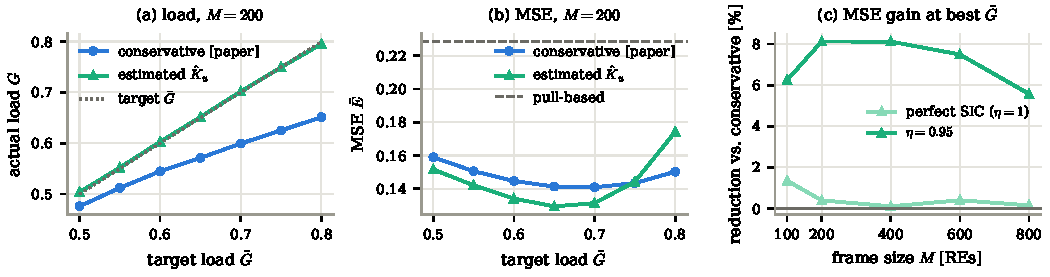
\includegraphics[width=\linewidth]{figs/synthetic.pdf}
  \caption{Effect of the count estimate on the Wiener model.
    (a,b)~$M=200$, $\eta=0.95$. The conservative update under-loads the channel; the
    estimated update reaches the target and lowers the MSE up to $\Gb\approx0.7$.
    (c)~MSE reduction at the best $\Gb$ ($Q_{95}$ in Table~\ref{tab}). The gain matters when unresolved
    frames are frequent (imperfect SIC).}
  \label{fig:synth}
\end{figure}

\paragraph{Effect of estimation.} On the Wiener model the beliefs are calibrated, and the
residual-power estimate removes the bias of Prop.~\ref{prop:excess}. The load rises from
\synLoadCons{} to \synLoadEst{} (target 0.70), and the MSE drops by up to
\synGainMaxImperfect\% with $\eta=0.95$ (Fig.~\ref{fig:synth}). With perfect SIC the gain is
at most \synGainMaxPerfect\%, because unresolved frames are rare. On this model calibration
adds nothing: the estimated update already reaches the target load.

\begin{figure}[t]
  \centering
  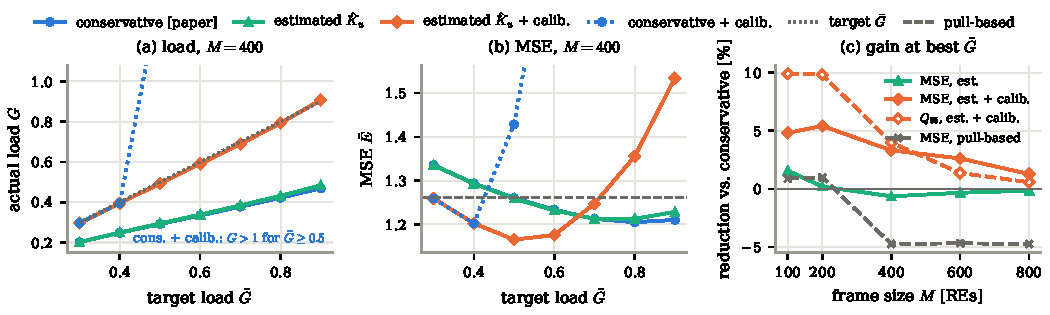
\includegraphics[width=\linewidth]{figs/real.pdf}
  \caption{Effect of calibration on smart-meter data (AR(1) model, $\eta=0.95$).
    (a)~Without calibration both updates reach little more than half of the target. Calibration with
    the estimated measurement tracks it; with the conservative measurement it overshoots.
    (b)~MSE at $M=400$. In this regime the uncalibrated scheme already beats pull-based polling
    (for $\Gb\ge0.6$), and calibration reaches a lower MSE at a lower target ($\Gb\approx0.5$).
    (c)~Reduction at the best $\Gb$ with respect to the conservative update. Estimation alone barely
    helps here; estimation and calibration together give the largest gain and beat pull-based in
    MSE at every $M$.}
  \label{fig:real}
\end{figure}

\paragraph{Effect of calibration.} On real data both updates are miscalibrated
(Fig.~\ref{fig:real}a). Estimation alone gains at most \realGainEstMax\%. With
calibration, the estimated measurement tracks the target (load \realLoadEstcFour{} at
$M=400$, $\Gb=0.7$), and the MSE falls by \realGainEstcMin--\realGainEstcMax\% and $Q_{95}$ by up to
\realGainQEstcMax\% (Table~\ref{tab}). Relative to pull-based polling, the MSE is lower by
\realVsPullMin--\realVsPullMax\%. For $M\ge400$ the uncalibrated scheme already beats
pull-based polling, by \realUncalVsPullMseMin--\realUncalVsPullMseMax\% in MSE and
\realUncalVsPullQMin--\realUncalVsPullQMax\% in $Q_{95}$, with the conservative or the estimated update alike.
It needs a nominal target of 0.8--1.0 to get there, because its actual load is only about 55--60\% of the nominal one. Calibration
widens the margin to \realCalVsPullMseMin--\realCalVsPullMseMax\% (MSE) and
\realCalVsPullQMin--\realCalVsPullQMax\% ($Q_{95}$). For $M\le200$, uncalibrated GO-IRSA is
within about 1\% of pull-based in MSE and worse in $Q_{95}$ at $M=100$. Only the calibrated scheme beats
it there in MSE, while at $M=100$ pull-based keeps a slightly lower $Q_{95}$.
Calibrating with the conservative measurement is
unstable: the load reaches up to \realLoadConscMax{} at the targets we tried.
Fig.~\ref{fig:trace} shows the dynamics behind Theorem~\ref{thm}. The per-frame load still swings
with the daily cycle, but its daily average stays on target, and the long-run error decays like
$1/T$. Without calibration it stalls at about $0.2$.

\begin{figure}[t]
  \centering
  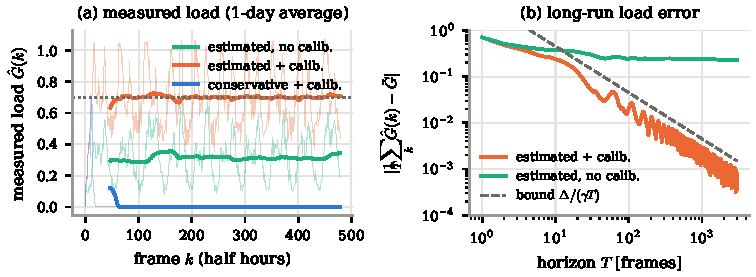
\includegraphics[width=0.72\linewidth]{figs/trace.pdf}
  \caption{Calibration dynamics on smart-meter data ($M=200$, $\eta=0.95$, $\Gb=0.7$,
    3000 frames, mean over 8 runs). (a)~Measured load per frame (thin) and its one-day
    average (thick). (b)~Long-run error of the measured load and the bound of
    Theorem~\ref{thm}, with $\Delta$ the largest observed deviation $|\Ge(k)-\Ge(1)|$.}
  \label{fig:trace}
\end{figure}

\begin{table}[t]
  \centering
  \caption{Reduction (\%) with respect to the conservative update, each method at its best
    target load. Positive values mean lower error.}
  \label{tab}
  \small
  \begin{tabular}{@{}lrrrr@{}}
\toprule
 & $M=100$ & $M=200$ & $M=400$ & $M=800$ \\
\midrule
\multicolumn{5}{@{}l}{\emph{Wiener model, $\eta=1$}} \\
\quad MSE, estimated & +1.3 & +0.4 & +0.1 & +0.1 \\
\quad $Q_{95}$, estimated & +1.3 & +0.4 & +0.1 & +0.1 \\
\multicolumn{5}{@{}l}{\emph{Wiener model, $\eta=0.95$}} \\
\quad MSE, estimated & +6.2 & +8.1 & +8.1 & +5.6 \\
\quad $Q_{95}$, estimated & +6.1 & +7.9 & +7.8 & +5.5 \\
\multicolumn{5}{@{}l}{\emph{Smart-meter data, $\eta=1$}} \\
\quad MSE, estimated & +1.7 & +0.6 & -0.3 & -0.5 \\
\quad MSE, estimated + calib. & +5.0 & +5.8 & +3.4 & +0.7 \\
\quad $Q_{95}$, estimated + calib. & +10.1 & +10.4 & +3.3 & +0.6 \\
\multicolumn{5}{@{}l}{\emph{Smart-meter data, $\eta=0.95$}} \\
\quad MSE, estimated & +1.6 & +0.2 & -0.6 & -0.1 \\
\quad MSE, estimated + calib. & +4.8 & +5.4 & +3.3 & +1.3 \\
\quad $Q_{95}$, estimated + calib. & +9.9 & +9.8 & +4.0 & +0.6 \\
\bottomrule
\end{tabular}

\end{table}

%======================================================================
\section{Real-time data: vehicle speeds}
\label{sec:ngsim}
%======================================================================
\paragraph{Setup.} NGSIM vehicle trajectories (US DOT, CC BY-SA 3.0): speeds at 10\,Hz on the
US-101 freeway and on Lankershim Boulevard\footnote{The I-80 part of the open export is incomplete.
Peachtree Street was excluded because its speeds lose their memory within one frame
($a=0.94$ per $0.1$\,s).}. Here \emph{one sample is one slot} ($0.1$\,s), which is the real-time
regime of the paper: the process evolves inside the frame, and a reading keeps 80--100\% of its
value over one frame. The model is an AR(1) per site, fitted on the first 30\% of each recording
($a=1$ on US-101, a random walk; $a=0.9975$ on Lankershim). The residuals are very heavy-tailed,
from lane changes and tracking jumps (excess kurtosis 29--110). Vehicles enter and leave: a node
slot is reused by the next vehicle, which registers its speed on entry. Seven time windows per
site run in parallel, so that about 2000 vehicles are present at any time. We use 30 episodes of
6\,min, $\Gb\in\{0.1,\dots,1.0\}$ and $\eta=0.95$; the pull-based baseline polls the $M$ present
vehicles with the largest model error variance.

\begin{figure}[t]
  \centering
  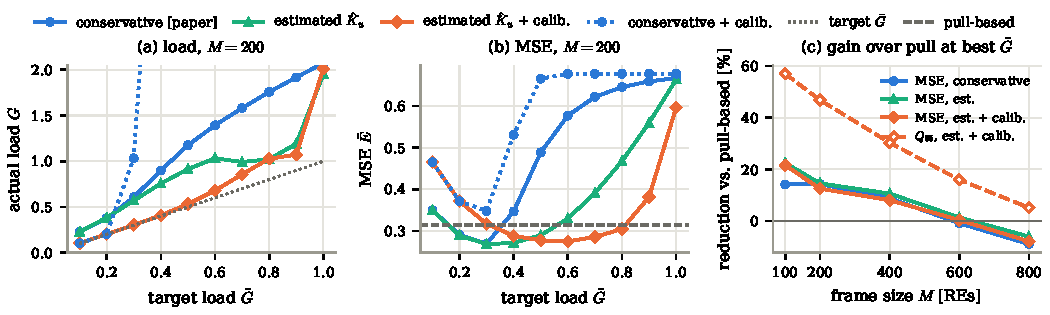
\includegraphics[width=\linewidth]{figs/ngsim.pdf}
  \caption{Vehicle speeds (NGSIM, $\eta=0.95$). (a)~The model underestimates the load:
    without calibration the channel is over-loaded and IRSA collapses. Calibration with the
    estimated measurement follows the target up to $\Gb\approx0.6$; with the conservative
    measurement it diverges. (b)~MSE at $M=200$. Calibration keeps the MSE near its minimum over
    a wide range of targets; without it, only a narrow, low nominal target works. (c)~Reduction
    with respect to pull-based polling at the best $\Gb$ of each method.}
  \label{fig:ngsim}
\end{figure}

\paragraph{Results.} Push-based access pays off clearly in this regime (Fig.~\ref{fig:ngsim}c).
At the best target load and for $M\le400$, every GO-IRSA variant beats pull-based polling, by
\ngVsPullMseMin--\ngVsPullMseMax\% in MSE and \ngVsPullQMin--\ngVsPullQMax\% in $Q_{95}$. The
vehicles whose speed suddenly changes report at once, which round-robin polling cannot do. At $M=800$ pull-based
is better in MSE (by \ngPullBetterMseMin--\ngPullBetterMseMax\%), but GO-IRSA keeps a lower
$Q_{95}$ (by \ngVsPullQEightMin--\ngVsPullQEightMax\%). The count estimate helps for short frames,
where unresolved frames are frequent: at $M=100$ it lowers the MSE by \ngEstGainMseHundred\% and $Q_{95}$ by
\ngEstGainQHundred\%.

Because the model \emph{under}estimates the load, the uncalibrated schemes reach their best
error only at a nominal target of about 0.3. With such a target the actual load is already about twice as
large (0.50--0.61; Fig.~\ref{fig:ngsim}a), and finding that target required tuning on the data. At its own best
target, calibration does not lower the error further (\ngCalGainMseMin\ to \ngCalGainMseMax\% in MSE for $M\ge200$),
because a detuned constant target compensates a roughly constant bias. Its benefit is
\emph{robustness}. The MSE stays within 5\% of its minimum for $\Gb\in$ \ngWinEstc{} with
calibration, against \ngWinCons{} (conservative) and \ngWinEst{} (estimated) without it. At the
nominal target $\Gb=0.7$, the MSE is \ngMseSevenEstcMin--\ngMseSevenEstcMax{} with calibration,
against \ngMseSevenConsMin--\ngMseSevenConsMax{} for the conservative update. Two limitations remain.
In deep collisions the residual-power estimate under-counts the undecoded transmitters, so the
calibrated load still overshoots slightly at small $M$ (\ngLoadEstc{} at $M=200$, $\Gb=0.7$).
Calibration with the conservative measurement diverges, as predicted by Assumption~\ref{ass}.

%======================================================================
\section{Conclusions}
%======================================================================
Two corrections make the GO-IRSA control loop unbiased. First, conditioning the beliefs on the number
of undecoded transmitters, estimated from residual power after SIC, removes the excess
belief mass left by unresolved frames; this matters when SIC is imperfect. Second, an online
calibration of the load target, driven by the same measurement, keeps the long-run load on
target with an $O(1/T)$ guarantee, even when the process model is wrong. The two depend on each
other: calibration is stable only with a measurement that counts the undecoded transmitters.
Calibration handles both directions of model error. When the beliefs overestimate the load (smart
meters), it recovers the unused capacity and lowers the error. When they underestimate it (vehicle
speeds), it prevents the collapse of IRSA and removes the need to tune the nominal target offline.

\begin{thebibliography}{9}
\bibitem{gibbs2021aci}
I.~Gibbs and E.~Cand\`es, ``Adaptive conformal inference under distribution shift,''
in \emph{Proc. NeurIPS}, 2021.
\bibitem{angelopoulos2023pid}
A.~N.~Angelopoulos, E.~J.~Cand\`es, and R.~J.~Tibshirani, ``Conformal PID control for time
series prediction,'' in \emph{Proc. NeurIPS}, 2023.
\end{thebibliography}

\end{document}
